\documentclass[10pt,a4paper]{article}

\usepackage{fontspec}
\setmainfont{Inter}[
  Path = /usr/share/fonts/rsms-inter-fonts/,
  Extension = .ttf,
  UprightFont = *-Regular,
  BoldFont = *-Bold,
  ItalicFont = *-Italic,
  BoldItalicFont = *-BoldItalic
]
\setmonofont{LiberationMono}[
  Path = /usr/share/fonts/liberation-mono-fonts/,
  Extension = .ttf,
  UprightFont = *-Regular,
  BoldFont = *-Bold,
  ItalicFont = *-Italic,
  BoldItalicFont = *-BoldItalic,
  Scale = 0.85
]

\usepackage[margin=1.8cm,top=2.2cm,bottom=2.1cm,headheight=20pt]{geometry}
\usepackage{graphicx}
\usepackage{xcolor}
\usepackage{colortbl}
\usepackage{booktabs}
\usepackage{tabularx}
\usepackage{longtable}
\usepackage{array}
\usepackage{pdflscape}
\usepackage{enumitem}
\usepackage{fancyhdr}
\usepackage{titlesec}
\usepackage{hyperref}

% ==================== PALETA KOLORÓW (SPÓJNA Z DIAGRAMAMI) ====================
\definecolor{Navy}{HTML}{1E3A5F}
\definecolor{LightBlue}{HTML}{EAF2FA}
\definecolor{SoftGreen}{HTML}{E6F4EA}
\definecolor{DarkGreen}{HTML}{2E7D32}
\definecolor{WarmBg}{HTML}{FFFBEB}
\definecolor{WarmBorder}{HTML}{D97706}
\definecolor{Slate}{HTML}{475569}
\definecolor{RowAlt}{HTML}{F8FAFC}
\definecolor{BorderGray}{HTML}{CBD5E1}

\hypersetup{
  colorlinks=true,
  linkcolor=Navy,
  urlcolor=Navy,
  pdftitle={MovieMatch — Laboratorium nr 7: Modelowanie UML},
  pdfauthor={Zespół MovieMatch — Inżynieria Oprogramowania UWM}
}

% ==================== NAGŁÓWKI I STOPKI ====================
\pagestyle{fancy}
\fancyhf{}
\fancyhead[L]{\small\color{Slate}\textbf{MovieMatch (MVP v1.0)} — Modelowanie systemu za pomocą diagramów UML}
\fancyhead[R]{\small\color{Slate}Inżynieria oprogramowania · Lab nr 7}
\fancyfoot[L]{\small\color{Slate}Uniwersytet Warmińsko-Mazurski w Olsztynie · WMiI}
\fancyfoot[R]{\small\color{Slate}Strona \thepage}
\renewcommand{\headrulewidth}{0.4pt}
\renewcommand{\footrulewidth}{0.4pt}
\renewcommand{\headrule}{\hbox to\headwidth{\color{BorderGray}\leaders\hrule height \headrulewidth\hfill}}
\renewcommand{\footrule}{\hbox to\headwidth{\color{BorderGray}\leaders\hrule height \footrulewidth\hfill}}

% ==================== STYLE SEKCJI ====================
\titleformat{\section}
  {\Large\bfseries\color{Navy}}
  {\thesection.}{0.5em}{}[\vspace{2pt}{\color{Navy}\titlerule[0.8pt]}]
\titleformat{\subsection}
  {\large\bfseries\color{Navy}}
  {\thesubsection.}{0.5em}{}

\setlength{\parindent}{0pt}
\setlength{\parskip}{5pt}
\setlist[itemize]{leftmargin=1.5em, itemsep=2pt, topsep=3pt}
\setlist[enumerate]{leftmargin=1.6em, itemsep=3pt, topsep=3pt}
\renewcommand{\arraystretch}{1.28}
\sloppy

% Pomocnicze ramki
\newcommand{\calloutbox}[3]{%
  \vspace{4pt}
  \noindent\fcolorbox{#1}{#2}{%
    \begin{minipage}{\dimexpr\textwidth-2\fboxsep-2\fboxrule\relax}
      #3
    \end{minipage}%
  }
  \vspace{4pt}
}

\begin{document}

% ==================== BANER TYTUŁOWY ====================
\thispagestyle{plain}
\noindent\colorbox{Navy}{%
  \begin{minipage}{\dimexpr\textwidth-2\fboxsep\relax}
    \vspace{10pt}
    \hspace{8pt}{\color{white}\small INŻYNIERIA OPROGRAMOWANIA (2026–2027) · UNIWERSYTET WARMIŃSKO-MAZURSKI W OLSZTYNIE}\\[4pt]
    \hspace{8pt}{\color{white}\LARGE\bfseries Modelowanie systemu MovieMatch (UML)}\\[4pt]
    \hspace{8pt}{\color{LightBlue}\normalsize Laboratorium nr 7 — Od wymagań do implementacji (Aplikacja webowa mobile-first, MVP v1.0)}
    \vspace{10pt}
  \end{minipage}%
}

\vspace{10pt}

\calloutbox{BorderGray}{LightBlue}{%
  \textbf{Cel opracowania:} Przygotowanie modelu kontekstowego oraz czterech wzajemnie spójnych diagramów UML (\textit{Activity}, \textit{Sequence}, \textit{State}, \textit{Class}) dla responsywnej aplikacji webowej (\textit{mobile-first approach}) \textbf{MovieMatch} (wersja MVP v1.0), weryfikacja ich zgodności z aktualną dokumentacją wymagań oraz zebranie kwestii do wyjaśnienia przed implementacją.\\[3pt]
  \textbf{Wybrany kluczowy scenariusz MVP:} \textit{Sesja grupowa i grupowe dobieranie filmu} (\texttt{FR-07}, \texttt{FR-06}, \texttt{FR-13}, \texttt{FR-10}, \texttt{US-4}, \texttt{US-5}).\\
  \textbf{Obiekt modelowany na diagramie stanu:} \texttt{Grupa} (sesja grupowa — tymczasowa 6h i stała).
}

\section{Zestawienie rezultatów laboratorium}

Wszystkie diagramy zostały wykonane w technologii \textbf{PlantUML} (kody źródłowe w katalogu \texttt{puml/}) i wyeksportowane zarówno jako wektorowe pliki \texttt{pdf/}, jak i obrazy wysokiej rozdzielczości \texttt{png/}.

\begin{table}[h!]
\centering
\small
\begin{tabularx}{\textwidth}{>{\bfseries}c >{\raggedright\arraybackslash}p{4.0cm} >{\raggedright\arraybackslash}X >{\raggedright\arraybackslash}p{4.7cm}}
\toprule
\rowcolor{Navy}
{\color{white}Nr} & {\color{white}\textbf{Wymagany rezultat}} & {\color{white}\textbf{Zakres w projekcie MovieMatch}} & {\color{white}\textbf{Pliki wyjściowe}} \\
\midrule
1 & Model kontekstowy (Context Diagram) & Granica aplikacji webowej (\textit{mobile-first}) i backendu MVP v1.0, 4 aktorów, przeglądarka WWW (HTTPS), komunikator, API filmów, backup & \texttt{01\_context\_diagram.pdf/.png} \\
\rowcolor{RowAlt}
2 & Activity Diagram & Przepływ sesji grupowej w 3 swimlane'ach: link przez Messenger, 3 ścieżki alternatywne, pętla maratonu i timeout 6h grupy tymczasowej & \texttt{02\_activity\_diagram.pdf/.png} \\
3 & Sequence Diagram & Chronologiczna komunikacja (55 komunikatów, 6 linii życia, klient webowy HTTPS, link URL poza aplikacją, maraton i timeout 6h) & \texttt{03\_sequence\_diagram.pdf/.png} \\
\rowcolor{RowAlt}
4 & State Diagram & Cykl życia obiektu \texttt{Grupa} (stan złożony + 7 stanów, maraton dla grup stałych/tymczasowych, wygasanie po 6h nieaktywności, usunięcie) & \texttt{04\_state\_diagram.pdf/.png} \\
5 & Class Diagram & 6 kluczowych klas dziedzinowych (w tym \texttt{nazwaUzytkownika} i \texttt{ostatniaAktywnoscO}), atrybuty, operacje, relacje, liczności i \texttt{\{xor\}} & \texttt{05\_class\_diagram.pdf/.png} \\
\rowcolor{RowAlt}
6 & Spójność i kwestie do wyjaśnienia & Matryca śledzenia FR/NFR, 6 uwag do spójności dokumentacji oraz 9 pytań biznesowych do PO & Sekcje 3, 4 i 5 niniejszego raportu \\
7 & Product Backlog (Jira) & Miejsce na link do backlogu z Lab 6 oraz oznaczenie pierwszej funkcjonalności do implementacji & Sekcja 6 niniejszego raportu \\
\bottomrule
\end{tabularx}
\end{table}

% ==================== SEKCJA 2: DIAGRAMY ====================
% --- LANDSCAPE PAGE: CONTEXT DIAGRAM ---
\begin{landscape}
\thispagestyle{fancy}
\section{Opracowane modele i diagramy UML}
\subsection{Model kontekstowy (Context Diagram)}
Model określa granicę systemu \textbf{MovieMatch (Aplikacja webowa \textit{mobile-first} + Backend, MVP v1.0)} bez projektowania szczegółów API. Wewnątrz granicy znajdują się wymagania wersji 1.0 (\texttt{FR-01}–\texttt{FR-04}, \texttt{FR-06}–\texttt{FR-08}, \texttt{FR-10}, \texttt{FR-11}, \texttt{FR-13}). Poza systemem wskazano 4 aktorów (z relacjami specjalizacji \texttt{Uczestnik} i \texttt{Administrator} względem \texttt{Użytkownika}) oraz 4 elementy otoczenia: \textbf{Przeglądarka WWW (Smartfon / Tablet / Desktop, HTTPS)}, \textbf{Zewnętrzny komunikator (np. Messenger / SMS)} do ręcznego przekazania wygenerowanego linku URL zaproszenia, \textbf{Zewnętrzna baza filmów (np. TMDB)} oraz \textbf{System kopii zapasowych (Backup Storage)}.
\vspace{4pt}
\begin{center}
  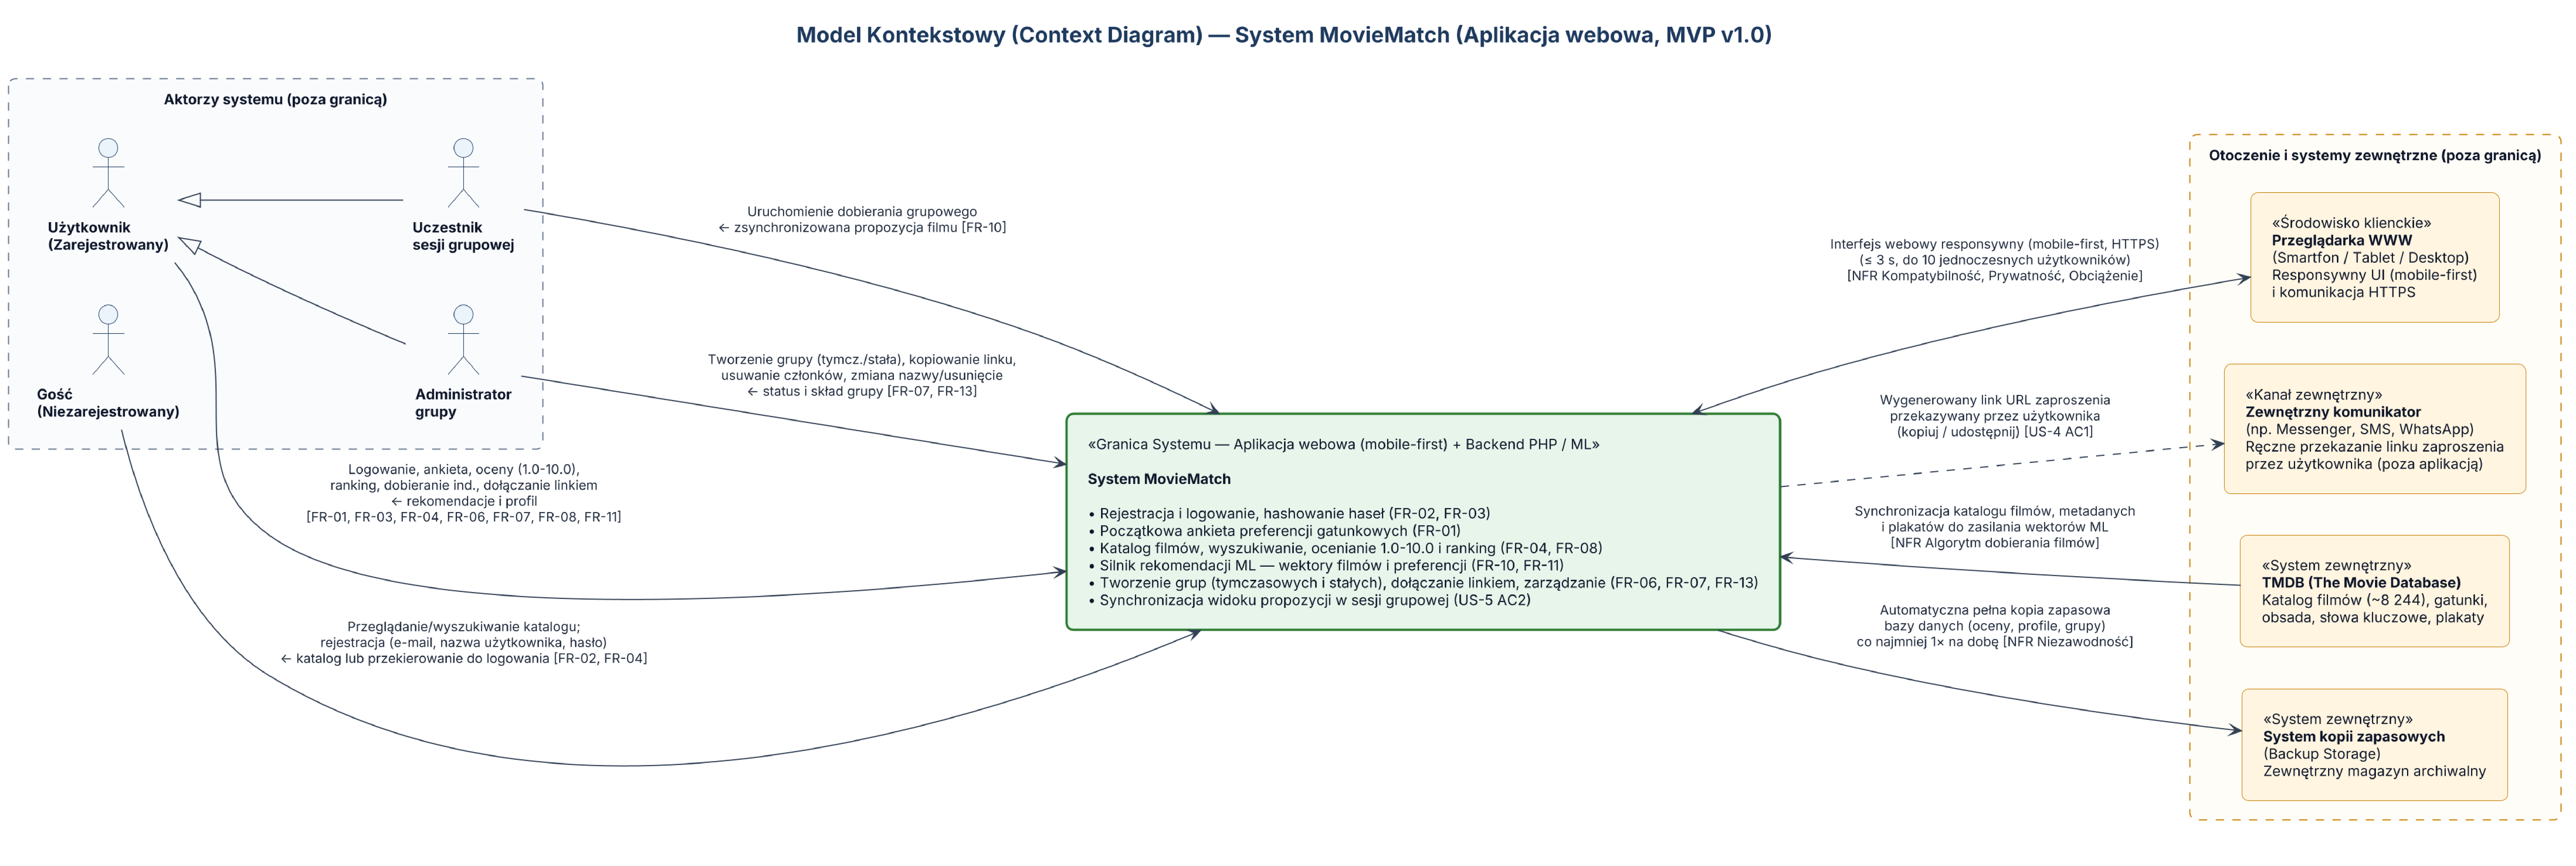
\includegraphics[width=\linewidth,height=0.69\textheight,keepaspectratio]{pdf/01_context_diagram.pdf}
\end{center}
\end{landscape}

\subsection{Diagram czynności (Activity Diagram)}
Diagram przedstawia przepływ scenariusza \textit{Sesja grupowa i grupowe dobieranie filmu} w 3 pasach odpowiedzialności (\texttt{Administrator grupy}, \texttt{System MovieMatch}, \texttt{Uczestnik sesji grupowej}). Administrator kopiuje i udostępnia wygenerowany link zaproszenia poza aplikacją (np. przez Messenger / SMS — \texttt{US-4 AC1}), a uczestnik otwiera go w przeglądarce (\texttt{FR-06}). Model zawiera 3 ścieżki alternatywne (niezalogowany gość, usunięcie uczestnika z pominięciem jego ocen, tryb awaryjny najwyższej średniej ocen w grupie) oraz pętlę ponownego dobierania (odrzucenie propozycji i maraton filmowy); grupa tymczasowa usuwa się automatycznie po \textbf{6 godzinach nieaktywności} (\texttt{FR-07}, \texttt{US-4 AC5}).

\begin{center}
  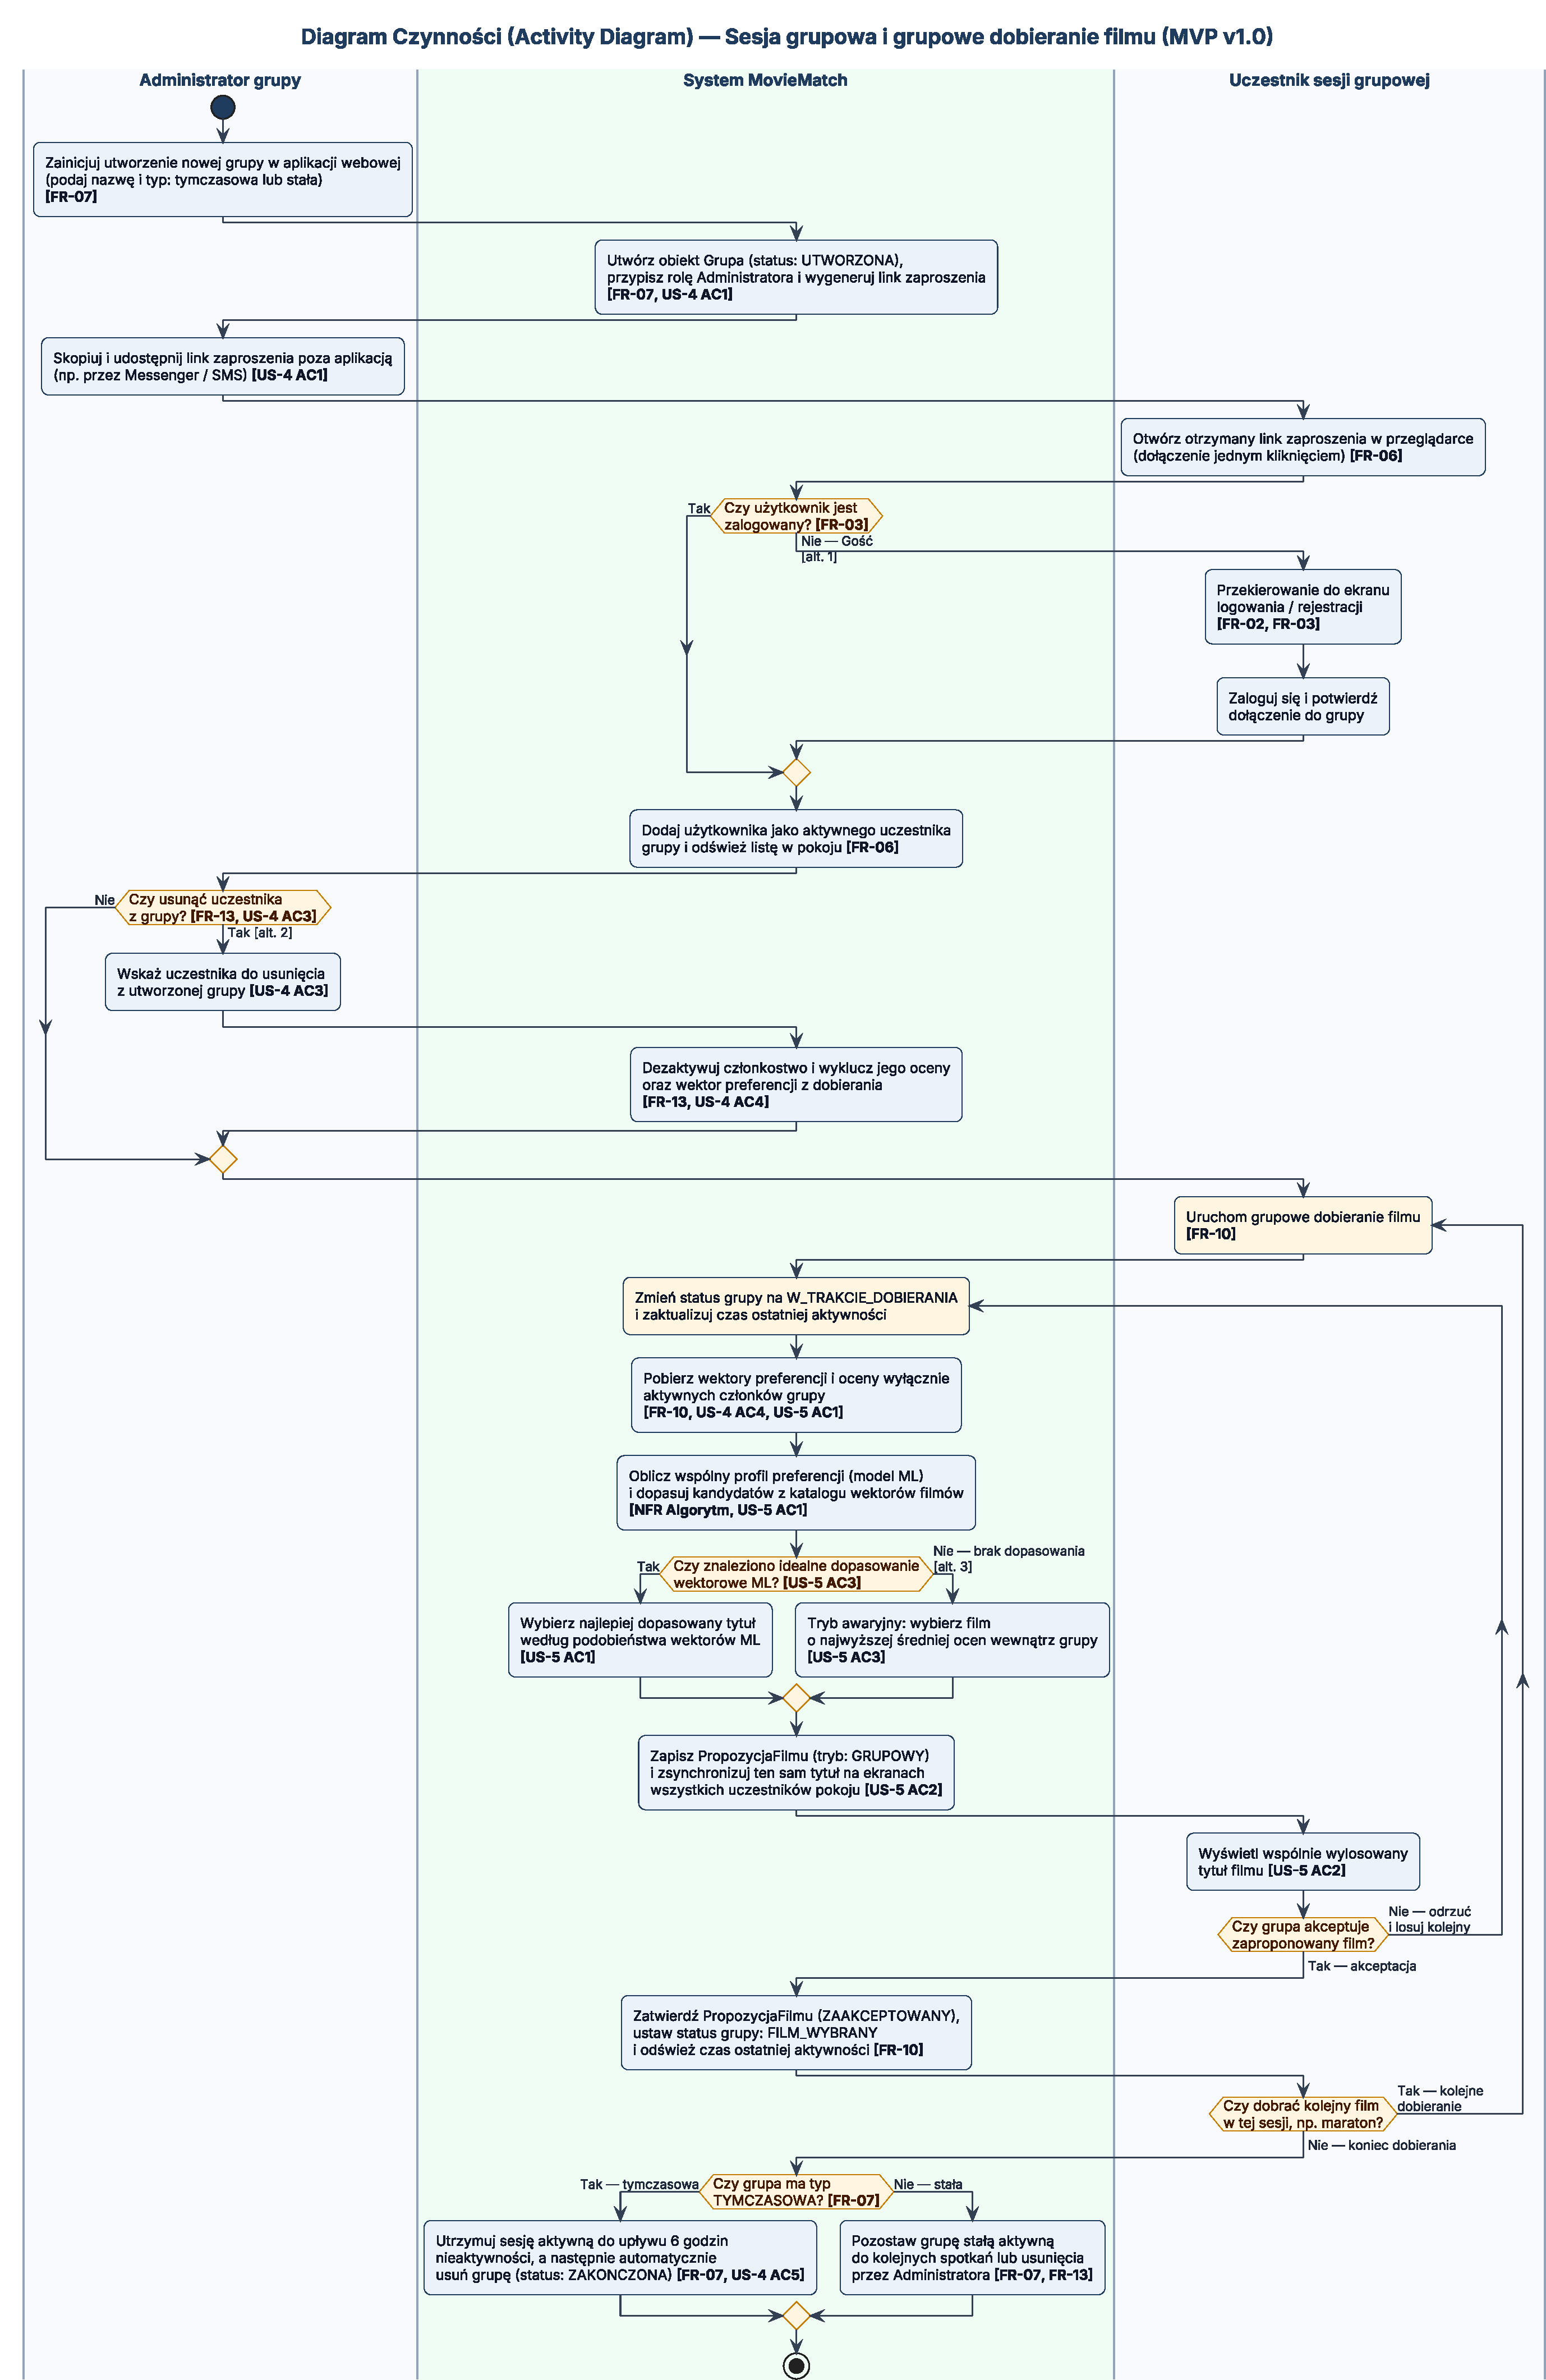
\includegraphics[width=\textwidth,height=0.75\textheight,keepaspectratio]{pdf/02_activity_diagram.pdf}
\end{center}

\newpage
\subsection{Diagram przebiegu (Sequence Diagram)}
Diagram opisuje \textbf{ten sam scenariusz} z perspektywy komunikacji w czasie pomiędzy 6 liniami życia (z klientem \texttt{Aplikacja Web (Klient HTTPS)}). Link zaproszenia jest przekazywany bezpośrednio między aktorami poza aplikacją (\texttt{[07]}), dołączenie następuje po otwarciu linku URL (\texttt{[08]}), a faza~5 uwzględnia zarówno możliwość dobrania kolejnego filmu (maraton), jak i automatyczne zamknięcie grupy tymczasowej po upływie \textbf{6 godzin nieaktywności} (\texttt{opt 6h}, \texttt{US-4 AC5}).

\begin{center}
  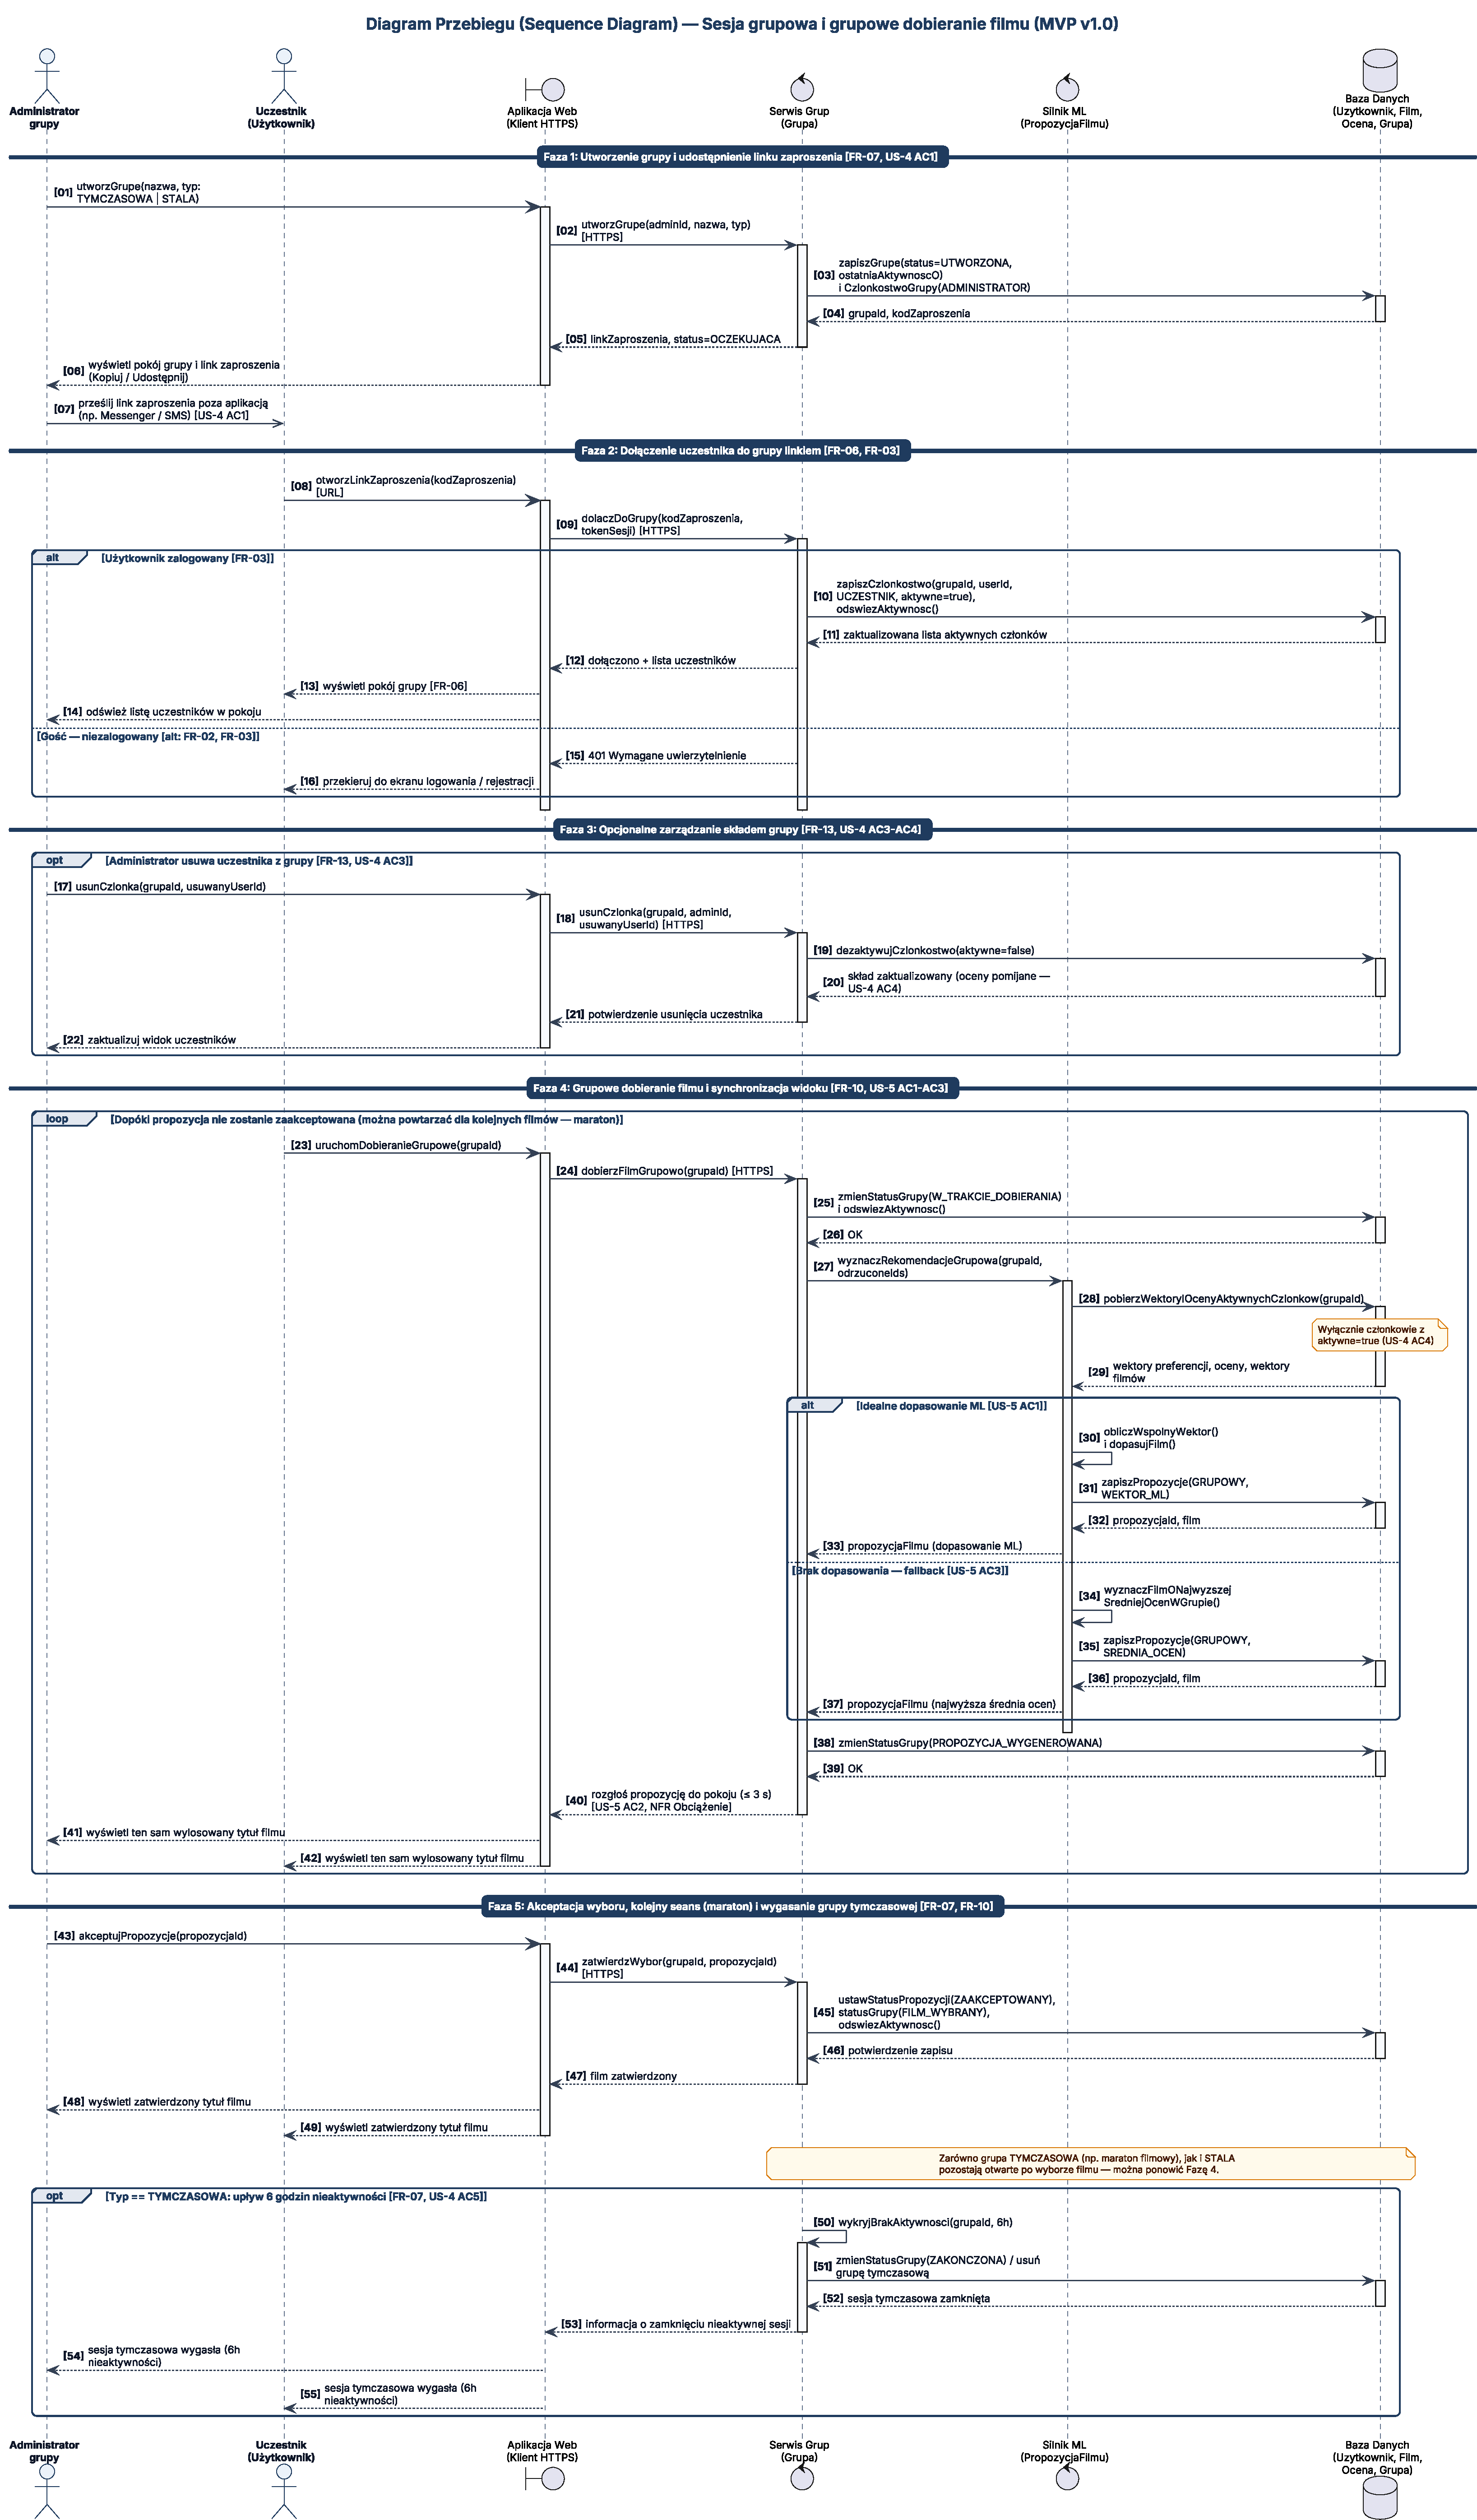
\includegraphics[width=\textwidth,height=0.79\textheight,keepaspectratio]{pdf/03_sequence_diagram.pdf}
\end{center}

\newpage
\subsection{Diagram stanu (State Diagram — obiekt \texttt{Grupa})}
Diagram modeluje cykl życia obiektu \texttt{Grupa} przy użyciu stanu złożonego \texttt{Aktywna Grupa} (5 stanów operacyjnych) oraz dwóch stanów końcowych: \texttt{ZAKONCZONA (Wygasła)} (dla grup typu \texttt{TYMCZASOWA} po zdarzeniu czasowym \texttt{after(6h nieaktywności)} — \texttt{FR-07}, \texttt{US-4 AC5}) oraz \texttt{USUNIETA (Anulowana)} (osiągalnego z dowolnego stanu aktywnego po wywołaniu \texttt{usunGrupe()} przez Administratora — \texttt{FR-13}). Przejście \texttt{FILM\_WYBRANY} $\to$ \texttt{OCZEKUJACA} wspiera kolejne dobierania (maraton filmowy) zarówno dla grup stałych, jak i tymczasowych.

\begin{center}
  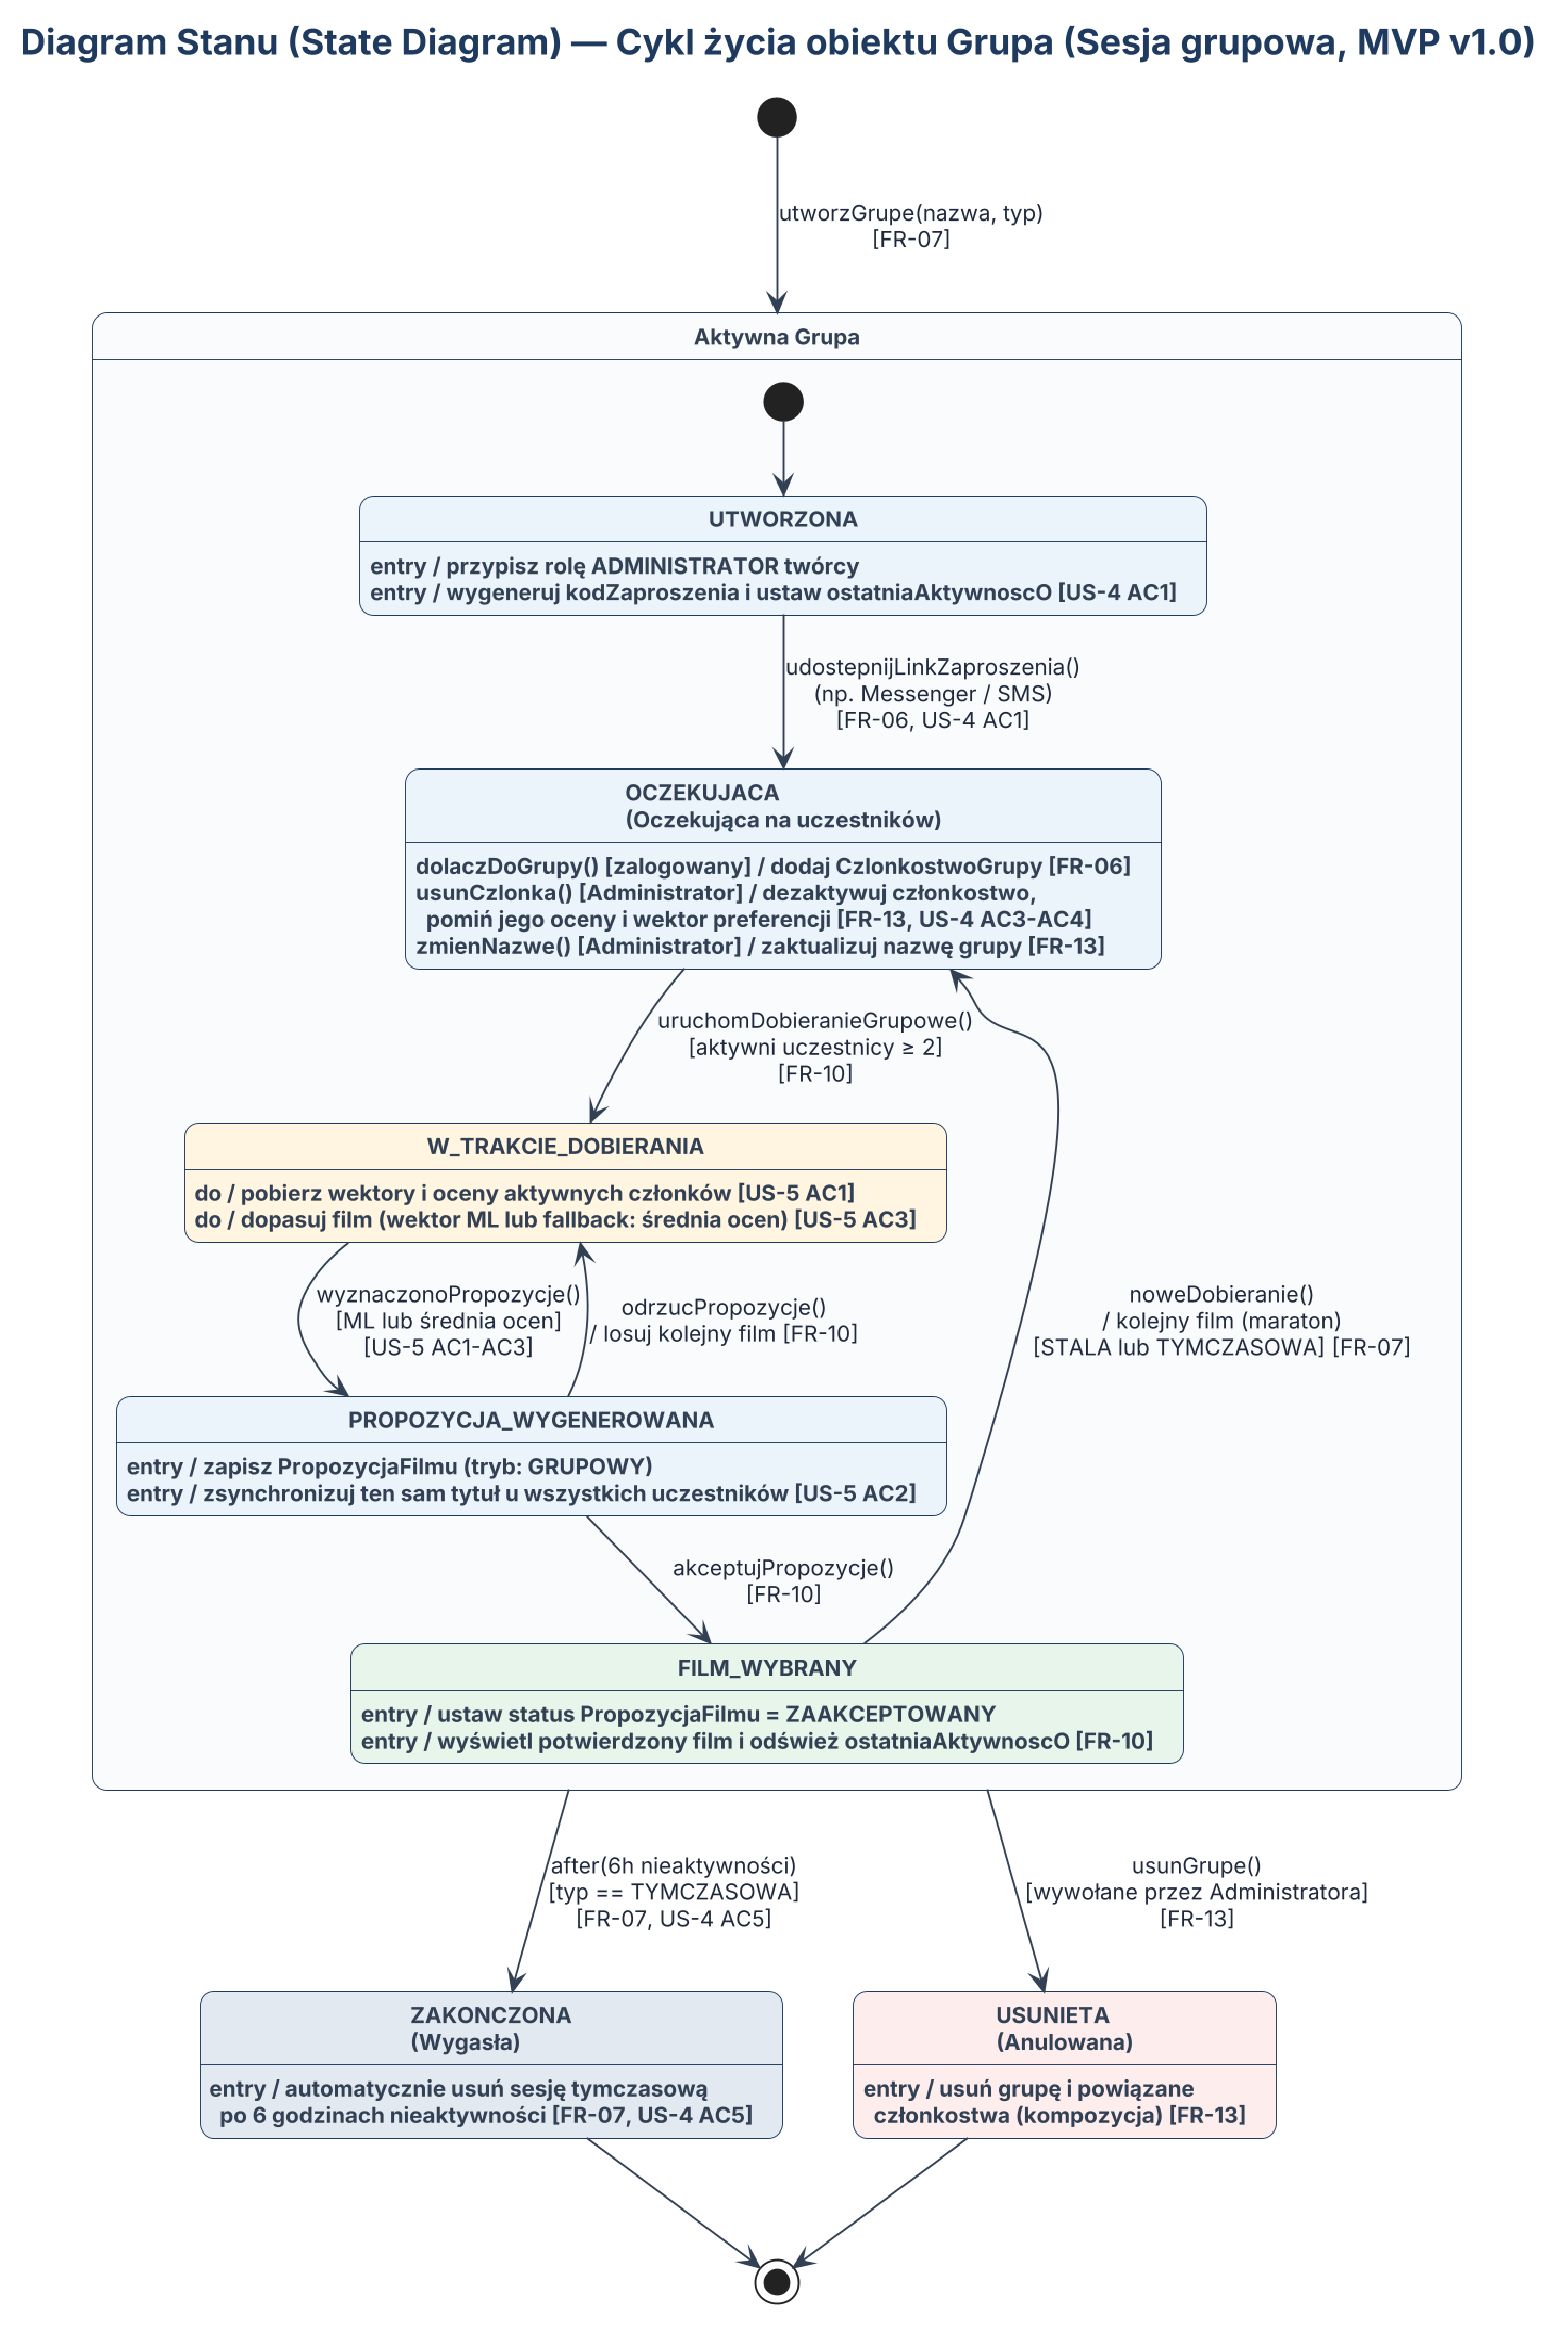
\includegraphics[width=\textwidth,height=0.76\textheight,keepaspectratio]{pdf/04_state_diagram.pdf}
\end{center}

% --- LANDSCAPE PAGE: CLASS DIAGRAM ---
\begin{landscape}
\thispagestyle{fancy}
\subsection{Diagram klas (Class Diagram — 6 kluczowych klas dziedzinowych)}
Struktura obejmuje 6 klas wynikających z wymagań MVP v1.0 (\texttt{Uzytkownik}, \texttt{Film}, \texttt{Ocena}, \texttt{Grupa} z polem \texttt{ostatniaAktywnoscO}, \texttt{CzlonkostwoGrupy}, \texttt{PropozycjaFilmu}) z pełnymi licznościami, kompozycją (\texttt{Grupa *-- CzlonkostwoGrupy}), agregacją (\texttt{Grupa o-- PropozycjaFilmu}) oraz ograniczeniami \texttt{\{xor\}} i unikalności pary \texttt{(Uzytkownik, Film)}.
\vspace{4pt}
\begin{center}
  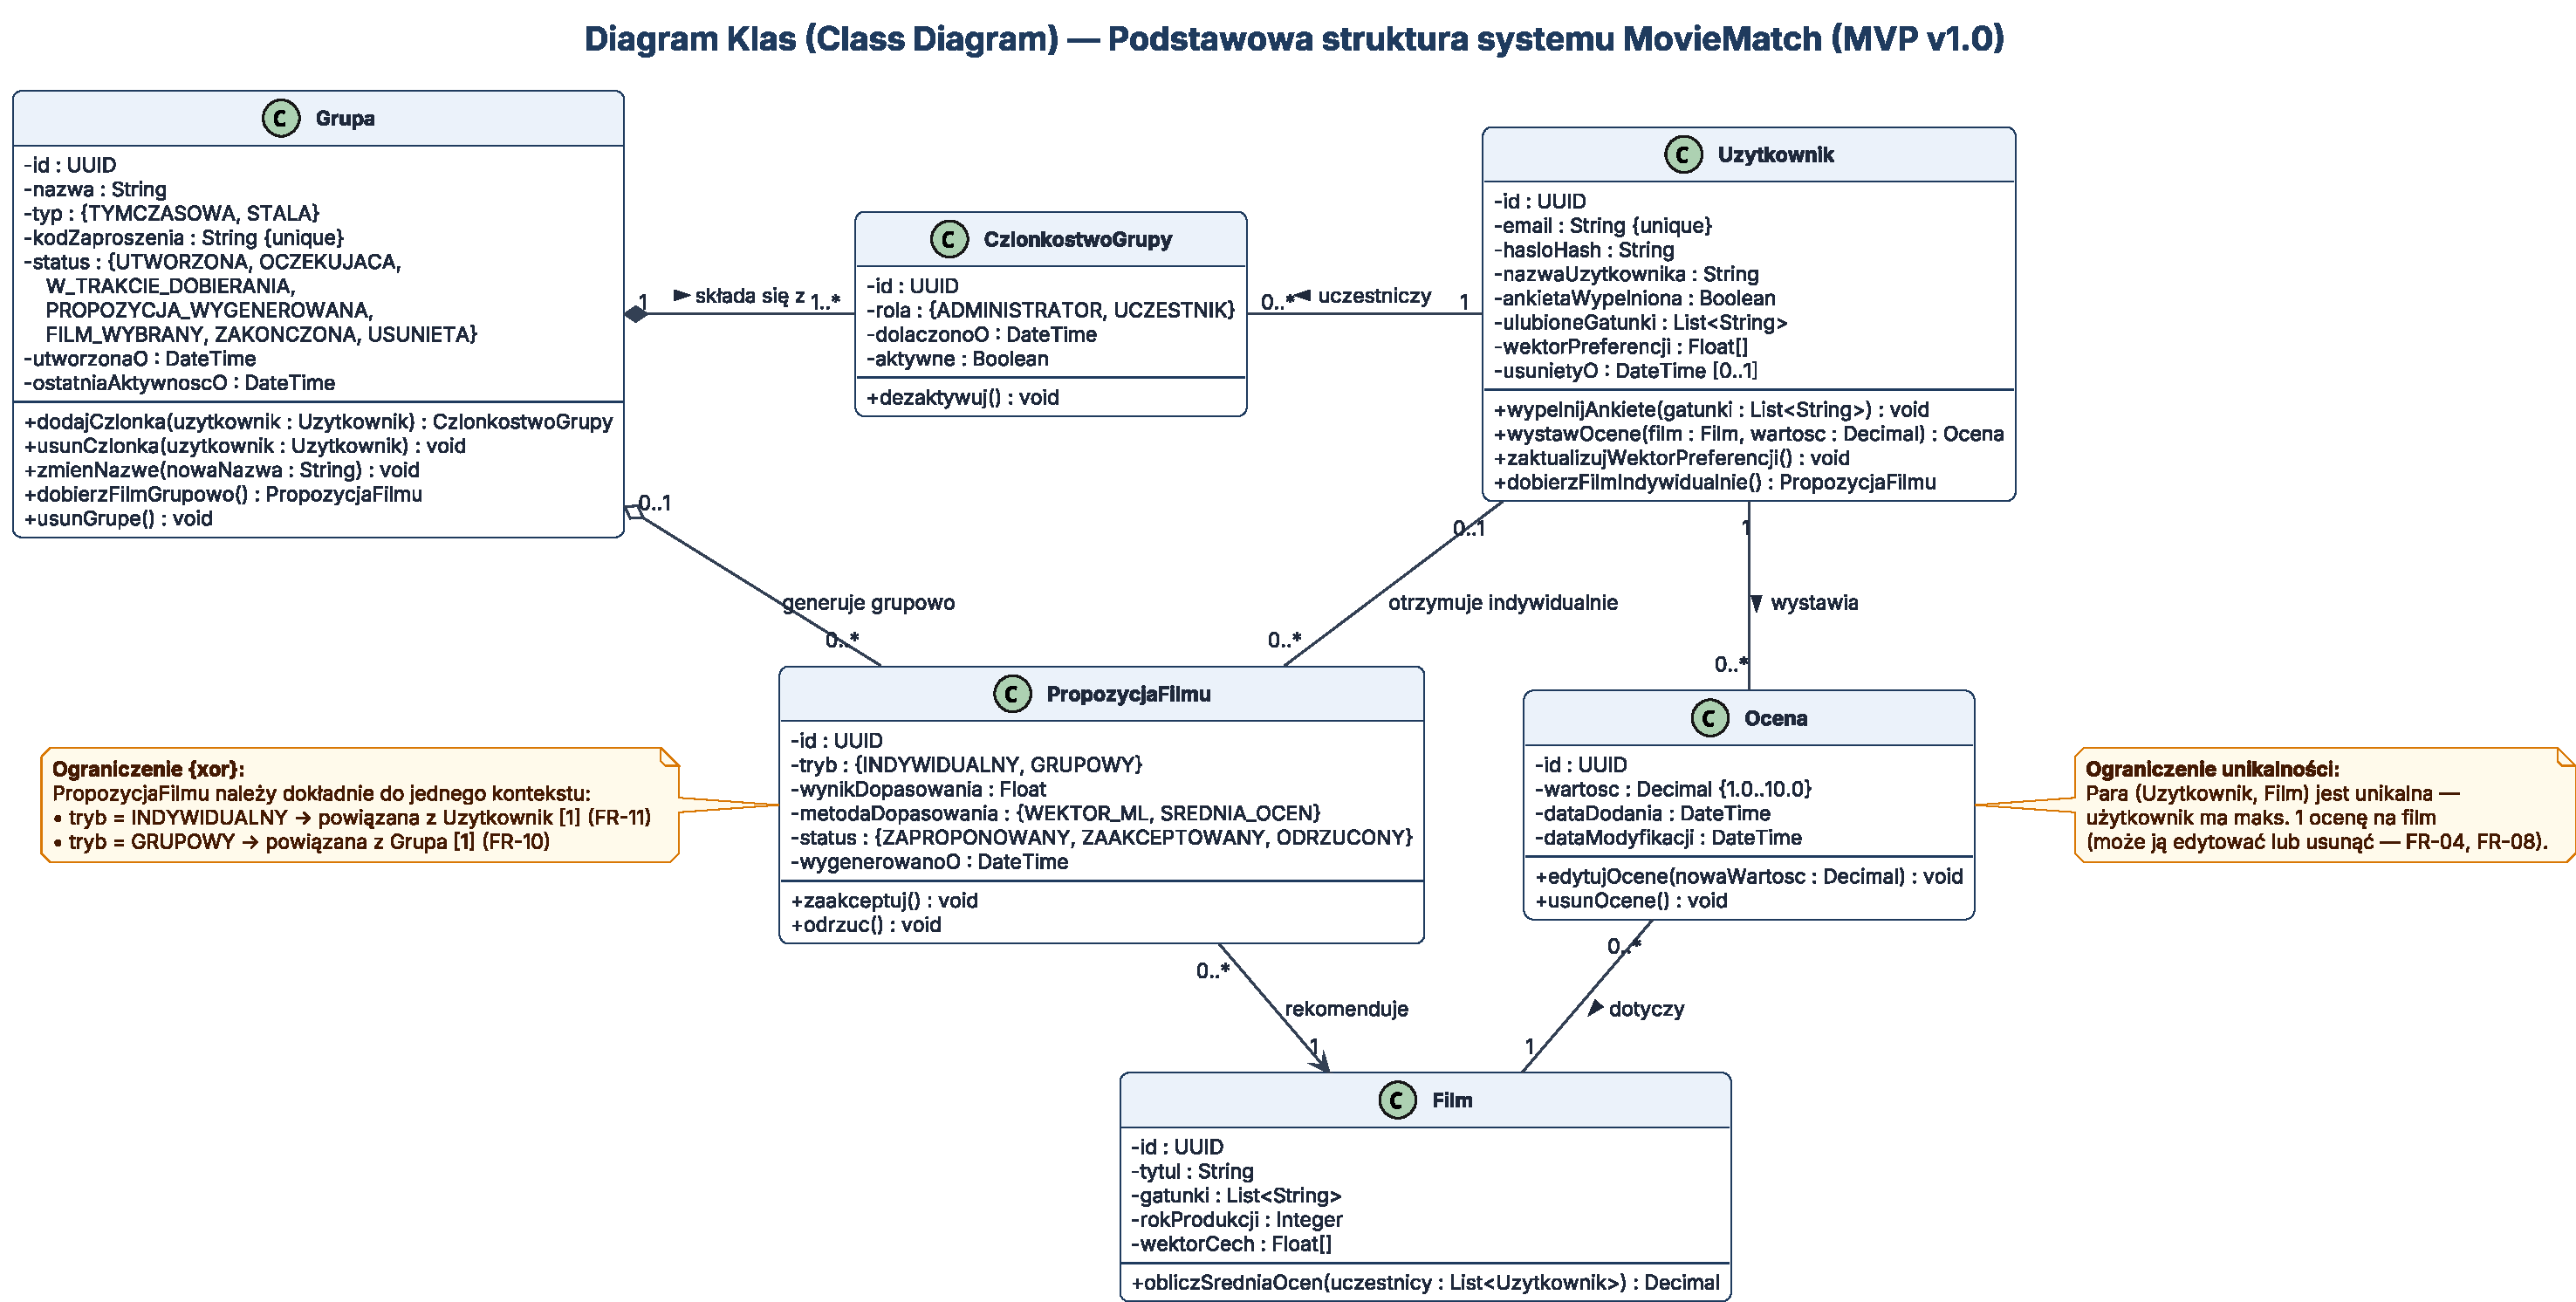
\includegraphics[width=\linewidth,height=0.76\textheight,keepaspectratio]{pdf/05_class_diagram.pdf}
\end{center}
\end{landscape}

% ==================== SEKCJA 3: MATRYCA SPÓJNOŚCI ====================
\section{Weryfikacja spójności modeli z wymaganiami (Matryca śledzenia)}

Poniższa matryca potwierdza pokrycie wymagań MVP v1.0 (FR oraz NFR) przez wszystkie pięć opracowanych modeli oraz spójność używanego słownictwa (identyczne nazwy klas, operacji, ról i statusów pomiędzy diagramami).

{\footnotesize
\setlength{\tabcolsep}{4pt}
\begin{longtable}{>{\raggedright\arraybackslash\bfseries}p{2.55cm} >{\raggedright\arraybackslash}p{2.4cm} >{\raggedright\arraybackslash}p{2.4cm} >{\raggedright\arraybackslash}p{2.4cm} >{\raggedright\arraybackslash}p{2.75cm} >{\raggedright\arraybackslash}p{3.15cm}}
\toprule
\rowcolor{Navy}
{\color{white}Wymaganie} & {\color{white}\textbf{Context}} & {\color{white}\textbf{Activity}} & {\color{white}\textbf{Sequence}} & {\color{white}\textbf{State (\texttt{Grupa})}} & {\color{white}\textbf{Class Diagram}} \\
\midrule
\endhead
\bottomrule
\endfoot
\texttt{FR-01} Ankieta początkowa (v1.0) & Zakres systemu, \texttt{Użytkownik} & \textit{(poza wybranym scenariuszem)} & \textit{(poza wybranym scenariuszem)} & — & \texttt{ankietaWypelniona}, \texttt{ulubioneGatunki}, \texttt{wypelnijAnkiete()} \\
\rowcolor{RowAlt}
\texttt{FR-02} Rejestracja (e-mail, nazwa, hasło) & Aktor \texttt{Gość} $\to$ System & Alt. 1 (przekierowanie Gościa) & \texttt{alt}: Gość $\to$ rejestracja & — & \texttt{email}, \texttt{nazwaUzytkownika}, \texttt{hasloHash} \\
\texttt{FR-03} Logowanie & Aktor \texttt{Użytkownik} & Decyzja: czy zalogowany? & Weryfikacja \texttt{tokenSesji}, \texttt{401} & Guard \texttt{[zalogowany]} & \texttt{Uzytkownik.email}, \texttt{hasloHash} \\
\rowcolor{RowAlt}
\texttt{FR-04} Ocenianie (1.0–10.0) & Przepływ ocen do systemu & Pobranie ocen aktywnych członków & Pobranie ocen z Bazy Danych & Aktywność w \texttt{W\_TRAKCIE\_\allowbreak DOBIERANIA} & \texttt{Ocena.wartosc} \{1.0..10.0\}, \texttt{wystawOcene()} \\
\texttt{FR-06} Dołączanie do grupy & \texttt{Użytkownik}, \texttt{Zewn. komunikator} & Otwarcie linku w przeglądarce (1 klik) & Link poza aplikacją (\texttt{[07]}) i Faza 2 (\texttt{[08]}–\texttt{[16]}) & \texttt{OCZEKUJACA}: \texttt{dolaczDoGrupy()} & \texttt{dodajCzlonka()}, \texttt{CzlonkostwoGrupy} \\
\rowcolor{RowAlt}
\texttt{FR-07} Tworzenie grupy (tymcz. 6h / stała) & \texttt{Administrator} $\to$ System & Start + maraton + usunięcie po 6h & Faza 1 (\texttt{[01]}–\texttt{[06]}) i Faza 5 (\texttt{opt 6h}) & \texttt{UTWORZONA}, maraton, \texttt{after(6h)} $\to$ \texttt{ZAKONCZONA} & \texttt{Grupa.typ}, \texttt{kodZaproszenia}, \texttt{ostatniaAktywnoscO} \\
\texttt{FR-08} Ranking filmów & Zakres systemu, \texttt{Użytkownik} & \textit{(poza wybranym scenariuszem)} & \textit{(poza wybranym scenariuszem)} & — & \texttt{Ocena.dataDodania}, \texttt{edytujOcene()}, \texttt{usunOcene()} \\
\rowcolor{RowAlt}
\texttt{FR-10} Dobieranie grupowo (\texttt{US-5}) & \texttt{Uczestnik} $\leftrightarrow$ System & Pętla ML + Alt. 3 (średnia) + sync & Faza 4 (\texttt{[23]}–\texttt{[42]}) i Faza 5 & \texttt{W\_TRAKCIE\_\allowbreak DOBIERANIA} $\to$ \texttt{PROPOZYCJA} $\to$ \texttt{FILM\_WYBRANY} & \texttt{PropozycjaFilmu} (\texttt{GRUPOWY}), \texttt{dobierzFilm\allowbreak Grupowo()} \\
\texttt{FR-11} Dobieranie indywidualne & \texttt{Użytkownik} $\leftrightarrow$ System & \textit{(poza wybranym scenariuszem)} & \textit{(poza wybranym scenariuszem)} & — & \texttt{PropozycjaFilmu} (\texttt{INDYWIDUALNY}), \texttt{dobierzFilm\allowbreak Indywidualnie()} \\
\rowcolor{RowAlt}
\texttt{FR-13} Zarządzanie grupą (\texttt{US-4}) & \texttt{Administrator} $\leftrightarrow$ System & Alt. 2: wyrzucenie i pominięcie ocen & Faza 3 \texttt{opt} (\texttt{[17]}–\texttt{[22]}) & \texttt{usunCzlonka()}, \texttt{zmienNazwe()}, \texttt{usunGrupe()} $\to$ \texttt{USUNIETA} & \texttt{usunCzlonka()}, \texttt{zmienNazwe()}, \texttt{usunGrupe()}, \texttt{aktywne} \\
\texttt{NFR} Kompat. (web), Bezp., Prywatność & \texttt{Przeglądarka WWW} (mobile-first, HTTPS) & Aplikacja webowa & \texttt{Aplikacja Web}, \texttt{[HTTPS]} & — & \texttt{hasloHash}, \texttt{usunietyO [0..1]} \\
\rowcolor{RowAlt}
\texttt{NFR} Obciążenie, Niezawodność, ML & Backup 1$\times$/dobę, Baza filmów, $\le 3$~s & Model ML (wektory) & Linia \texttt{Silnik ML}, czas $\le 3$~s & \texttt{do /} dopasowanie ML lub średnia & \texttt{wektorCech}, \texttt{wektorPreferencji} \\
\end{longtable}
}

% ==================== SEKCJA 4: SPÓJNOŚĆ DOKUMENTACJI ====================
\newpage
\section{Sprawdzenie spójności dokumentu wymagań (pozostałe uwagi)}

W zaktualizowanej dokumentacji poprawnie ujednolicono \texttt{FR-01} (dodano do MUST i usunięto sprzeczne wykluczenie), doprecyzowano formę aplikacji (\textit{webowa, mobile-first}), rozszerzono \texttt{FR-02} o nazwę użytkownika oraz określono 6-godzinny limit nieaktywności grupy tymczasowej (\texttt{FR-07}, \texttt{US-4 AC5}). Pozostają drobne niespójności w samym dokumencie:
\begin{enumerate}
  \item \textbf{\texttt{FR-02} vs \texttt{US-1} (str.~1 i~4):} \texttt{FR-02} wymaga teraz adresu e-mail, \textbf{nazwy użytkownika} i hasła, natomiast \texttt{US-1} nadal mówi wyłącznie o e-mailu i haśle (brakuje też kryterium akceptacji o walidacji/unikalności nazwy użytkownika).
  \item \textbf{\texttt{FR-06} i \texttt{US-4 AC1–AC2} (str.~1 i~4):} \texttt{US-4 AC2} nadal mówi o „powiadomieniu dla zaproszonych znajomych”, a \texttt{FR-06} o „grupie znajomych”, mimo że system znajomych (\texttt{FR-05}) jest dopiero w \texttt{v1.2}, a w MVP v1.0 link zaproszenia przekazywany jest zewnętrznie (np. przez Messenger).
  \item \textbf{NFR „Prywatność” bez odpowiadającego FR ani User Story (str.~3):} Sekcja~3 wymaga 24-godzinnego okna na cofnięcie usunięcia konta, lecz brakuje odpowiedniego FR oraz User Story.
  \item \textbf{Pomyłka numeracji w dzienniku zmian (str.~8, pkt~3):} Zapisano \textit{„Zmiana FR-11, dodanie opisu grup Tymczasowe i stałe”}, podczas gdy zmiana dotyczy \textbf{\texttt{FR-07}} (Tworzenie grupy), a \texttt{FR-11} to dobieranie indywidualne.
  \item \textbf{Nazewnictwo w \texttt{US-3} i zakres backupu w NFR „Niezawodność” (str.~3 i~4):} W \texttt{US-3} pozostało słowo „po loginie” (zamiast „nazwy użytkownika / kodu znajomego”), a NFR backupu wymienia jedynie oceny i listy znajomych (v1.2), pomijając konta, wektory preferencji i grupy z MVP v1.0.
  \item \textbf{Sekcja~6, pkt~2 (str.~7):} W opisie zakresu wersji 1.0 („Profilowanie i zbieranie preferencji”) warto obok oceniania filmów dopisać również wypełnianie początkowej ankiety (\texttt{FR-01}).
\end{enumerate}

% ==================== SEKCJA 5: PYTANIA DO PO ====================
\newpage
\section{Pytania i decyzje do wyjaśnienia z Product Ownerem}

Zgodnie z zasadą niezgadywania brakujących reguł biznesowych, przed rozpoczęciem implementacji zespół powinien uzyskać od Product Ownera rozstrzygnięcie poniższych 9 kwestii:

{\small
\setlength{\tabcolsep}{5pt}
\begin{longtable}{>{\bfseries}p{1.0cm} >{\raggedright\arraybackslash}p{2.4cm} >{\raggedright\arraybackslash}p{7.1cm} >{\raggedright\arraybackslash}p{5.2cm}}
\toprule
\rowcolor{Navy}
{\color{white}ID} & {\color{white}\textbf{Dotyczy}} & {\color{white}\textbf{Pytanie do Product Ownera}} & {\color{white}\textbf{Wpływ na modele / kod}} \\
\midrule
\endhead
\bottomrule
\endfoot
Q-01 & Context, Class & Skąd pochodzi katalog filmów: zewnętrzne API (np. TMDB) czy własny statyczny zbiór danych dla modelu ML? & Zależność zewnętrzna w Modelu kontekstowym i zasilanie \texttt{Film.wektorCech}. \\
\rowcolor{RowAlt}
Q-02 & Activity, Sequence (\texttt{US-5 AC3}) & Jaki próg podobieństwa wektorów uznajemy za „idealne dopasowanie”, poniżej którego włącza się tryb awaryjny (najwyższa średnia ocen w grupie)? & Warunek rozgałęzienia \texttt{alt} w \texttt{Silniku ML}. \\
Q-03 & Activity, Sequence (\texttt{FR-10} vs \texttt{FR-11}) & Czy w dobieraniu grupowym ML wykluczamy filmy już ocenione przez wszystkich członków, przez kogokolwiek, czy w ogóle ich nie wykluczamy? & Filtrowanie kandydatów w \texttt{wyznaczRekomendacje\allowbreak Grupowa()}. \\
\rowcolor{RowAlt}
Q-04 & Activity, Sequence, State & Kto w grupie może uruchomić losowanie, odrzucić propozycję i zaakceptować wybrany film — każdy uczestnik, tylko Administrator czy głosowanie wszystkich? & Kontrola uprawnień w \texttt{Serwisie Grup} i strażniki w \texttt{State Diagram}. \\
Q-05 & State, Sequence (\texttt{FR-07}, \texttt{FR-13}) & (a) Czy grupowe dobieranie wymaga min.~2 aktywnych członków? (b) Co dzieje się z grupą stałą po odejściu lub usunięciu konta Administratora? \textit{(Timeout grupy tymczasowej ustalono już na 6h w \texttt{US-4 AC5}).} & Strażnik \texttt{[aktywni $\ge$ 2]} i reguły przekazania/usunięcia grupy stałej. \\
\rowcolor{RowAlt}
Q-06 & Class, \texttt{FR-01} (\texttt{US-2 AC2}) & Jaka dokładnie jest minimalna wymagana liczba gatunków w początkowej ankiecie preferencji (np.~3)? & Walidacja formularza ankiety i inicjalizacja \texttt{wektorPreferencji}. \\
Q-07 & Class, \texttt{FR-08} (\texttt{US-8 AC3}) & Czy edycja lub usunięcie oceny w rankingu natychmiast przelicza wektor preferencji użytkownika (analogicznie do \texttt{US-7 AC3})? & Wywołanie \texttt{zaktualizuj\allowbreak WektorPreferencji()} w \texttt{Ocena}. \\
\rowcolor{RowAlt}
Q-08 & NFR Prywatność, Class & Czy usuwanie konta (z 24-godzinnym czasem na cofnięcie) wchodzi do MVP v1.0 — a jeśli tak, czy dopisujemy brakujące FR i US? & Zakres backlogu MVP i harmonogram czyszczenia danych. \\
Q-09 & Sequence (\texttt{US-5 AC2}), NFR & Czy synchronizację widoku pokoju w aplikacji webowej (maks.~10 osób, $\le 3$~s) realizujemy przez WebSocket/SSE czy cykliczny polling? & Architektura komunikacji w fazie~4 \texttt{Sequence Diagram}. \\
\end{longtable}
}

% ==================== SEKCJA 6: PRODUCT BACKLOG ====================
\newpage
\section{Link do Product Backlogu i pierwsza funkcjonalność}

\calloutbox{WarmBorder}{WarmBg}{%
  \textbf{Link do Product Backlogu zespołu (Jira — Lab 6):}\\[3pt]
  \texttt{[WKLEJ TUTAJ LINK DO PRODUCT BACKLOGU PROJEKTU MOVIEMATCH W JIRA]}\\[4pt]
  {\small\color{Slate}\textit{Uwaga: przed przesłaniem raportu na Teams uzupełnij powyższy link adresem tablicy Jira i upewnij się, że poniższa funkcjonalność startowa jest oznaczona na górze backlogu (np. etykietą \texttt{MVP-FIRST} / \texttt{Sprint 1}).}}
}

\subsection*{Oznaczona pierwsza funkcjonalność do implementacji}
Na podstawie analizy zależności wynikających z opracowanych diagramów UML (ścieżka alternatywna~1 w \textit{Activity Diagram} i blok \texttt{alt} w \textit{Sequence Diagram} pokazują, że brak uwierzytelnionego użytkownika blokuje zarówno ocenianie filmów, jak i dołączanie do sesji grupowych), jako pierwszą funkcjonalność w Product Backlogu wyznaczono:
\begin{itemize}
  \item \textbf{Start MVP (Sprint 1 — fundament odblokowujący cały system):} \textbf{\texttt{FR-02} Rejestracja konta + \texttt{FR-03} Logowanie użytkownika} (\texttt{US-1}, \texttt{US-6}, priorytet \texttt{Must}, wersja \texttt{1.0}, niskie ryzyko). Zapewnia obiekt \texttt{Uzytkownik} (\texttt{email}, \texttt{nazwaUzytkownika}, \texttt{hasloHash}) oraz sesję HTTPS, bez których nie mogą działać ankieta (\texttt{FR-01}), oceny (\texttt{FR-04}) ani grupy.
  \item \textbf{Kolejny priorytetowy przyrost (rdzeń biznesowy zamodelowany w Lab 7):} po dostarczeniu uwierzytelniania oraz ankiety/ocen (\texttt{FR-01}, \texttt{FR-04}) realizowany jest zamodelowany scenariusz \textbf{\texttt{FR-07} Tworzenie grupy $\to$ \texttt{FR-06} Dołączanie do grupy $\to$ \texttt{FR-10} Dobieranie grupowo filmu}.
\end{itemize}

\end{document}
